\documentclass[a4paper,12pt]{article}
\usepackage[latin1]{inputenc}
\usepackage[spanish]{babel}
\usepackage{bm}
\usepackage{graphicx}
\usepackage{amsmath}
\setlength{\textheight}{235mm}
\setlength{\textwidth}{168mm}
\setlength{\oddsidemargin}{0pt}
\pagestyle{empty}
\begin{document}
\mbox{}\vspace*{-45mm}

{\centering
{\small\sc Escuela T�cnica Superior de Ingenieros de Caminos, Canales y
Puertos (Madrid)}\\*[4mm]
{\Large\bf M�todo de los Elementos Finitos (Curso 22-23)}\\*[4mm]
Test 6: Beam models and static analysis\\*[4mm]

}

\vspace{3mm}

%%%%%
The two-span frame is made with reinforced concrete, with elastic module $E=32$ GPa, Poisson coefficient $\nu=0.20$, and mass density $\rho=2548.42$ kg/m$^3$. The beam cross-section is $0.30 m\times0.60$ m (width and height), and the column cross-section is square with $0.40$ m side. The loads in the structure are their own weight, the two vertical loads (at J and K), one horizontal load (at C) and one uniform vertical load (on the beams). The supports A, D and G are fully fixed.

Run the static analysis considering a 3D model, B31 element type, element size of $0.5$ m ($Global Seed/Approximate global size$) and answer the question of the quiz.
\\
\begin{center}
	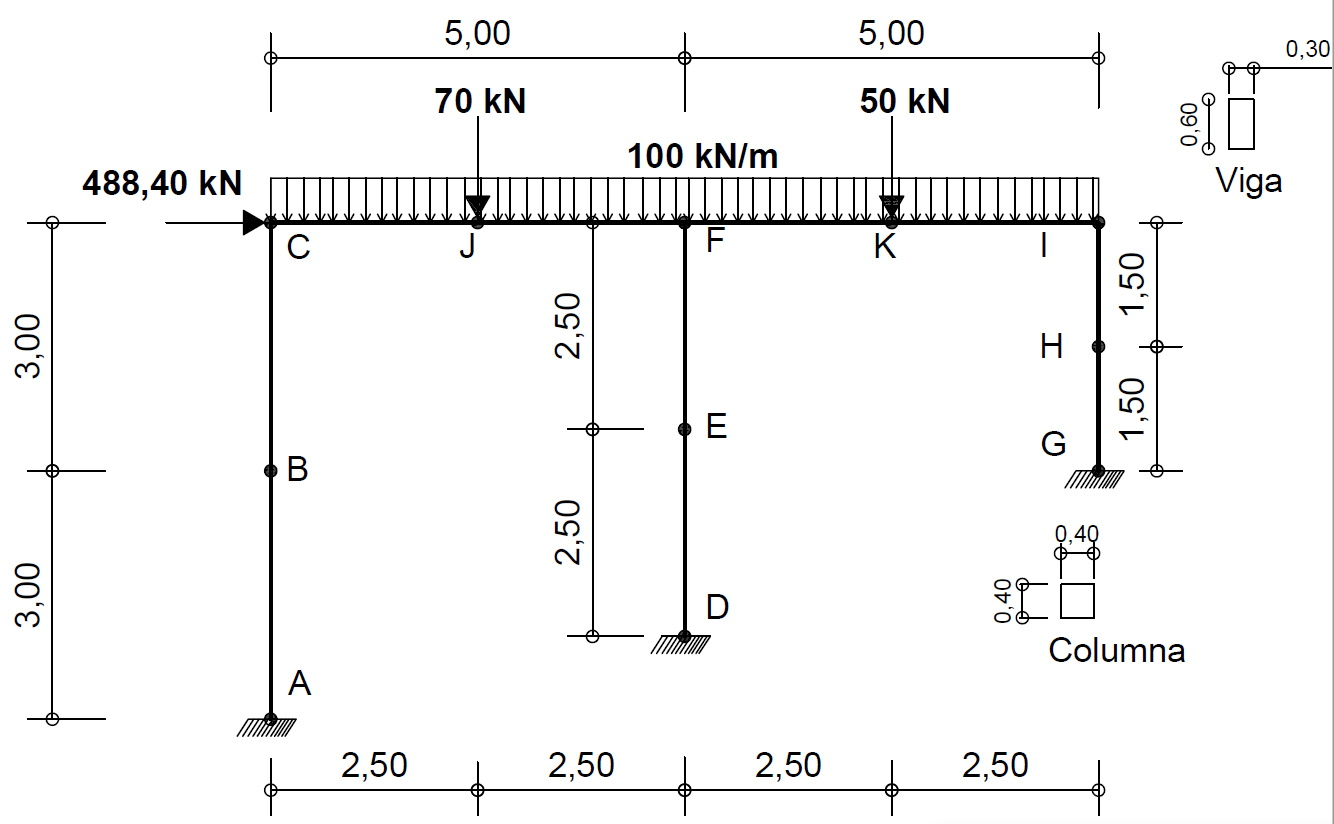
\includegraphics[width=1\textwidth]{figura5}
\end{center}
\end{document}
